
\documentclass{article}
\usepackage[utf8]{inputenc}
\usepackage{amsmath}

\usepackage{algorithm}
\usepackage{algorithmic}


\usepackage[english]{babel}
\usepackage[T1]{fontenc}
\usepackage{amsmath}
\usepackage{amsfonts}
\usepackage{amssymb}
\usepackage{csvsimple}





\usepackage{graphicx}


\newcommand{\vect}[1]{\ensuremath{\boldsymbol{\mathbf{#1}}}} 
\newcommand{\matr}[1]{\ensuremath{\boldsymbol{\mathbf{#1}}}}

\newcommand{\codevar}[1]{\textbf{#1}}



\usepackage{mathtools}
\DeclarePairedDelimiter\ceil{\lceil}{\rceil}
\DeclarePairedDelimiter\floor{\lfloor}{\rfloor}


\title{Exercise 3 - Spatial Statistics}
\author{Amir Ahmed}
\date{April 2020}


\begin{document}
	\maketitle
	
	\section*{Problem 1: Markov RF}
	Assume that we have observed seismic data over a domain $D \in \mathbb{R}^2$. We want to identify the underlying lithology distribution over D, the underlying lithology of a point is either sand or shale, $\lbrace 1, 0 \rbrace$ respectively.
	
	The observations have been collected on a regular $(75 \times 75)$ grid $L_d$, with seismic data being $\lbrace d(\vect x); \vect x \in L_d \rbrace$. Where $d(\vect x) \in \mathbb{R}$. 
	
	We have observed the lithology distribution in a geologically comparable domain $D_c \in \mathbb{R}^2$. Assume that this was collected on a regular $(66 \times 66)$ grid $L_{D_c}$. 
	
	We assume that the underlying lithology distribution can be represented by a Mosaic RF $\lbrace l(\vect x); \vect x \in  L_D\rbrace, l(\vect x) \in \lbrace 0, 1 \rbrace$.  
	
	
	\subsection*{Problem 1a)}
	 We start by looking at $L_d$.
	 Let the seismic data collection procedure follow the following likelihood model: 
	 $$\left[d_i | \vect l \right] = \begin{cases}
	 0.02 + U_i \text{ if sand, } l_i = 0 \\
	 0.08 + U_i \text{ if shale, } l_i = 1
	 \end{cases}$$
	 $i = 1, 2, \dots, n$. With $U_i$ being identically independently distributed $U_i \sim N(0, 0.06^2)$. This would make each observation point $d_i$ conditionally independent on $\vect l$. That will say: 
	\begin{equation}
		p(d_i | \vect l) = p(d_i | l_i) = \phi(d_i |\mu = 0.02 + 0.06l_i, \sigma^2 = 0.06^2)
	\end{equation}	
	 Where $\phi$ is the pdf of the normal distribution. As all observations are independent we thus have: 
	 \begin{equation}\label{eq:cond_prob}
	 	p(\vect d | \vect l) = \prod_{i=1}^{n}p(d_i | l_i) = \prod_{i=1}^{n}  \phi(d_i |\mu = 0.02 + 0.06l_i, \sigma^2 = 0.06^2)
	 \end{equation} 
	 
	 \begin{figure}[h]	
	 	\begin{center} 
	 		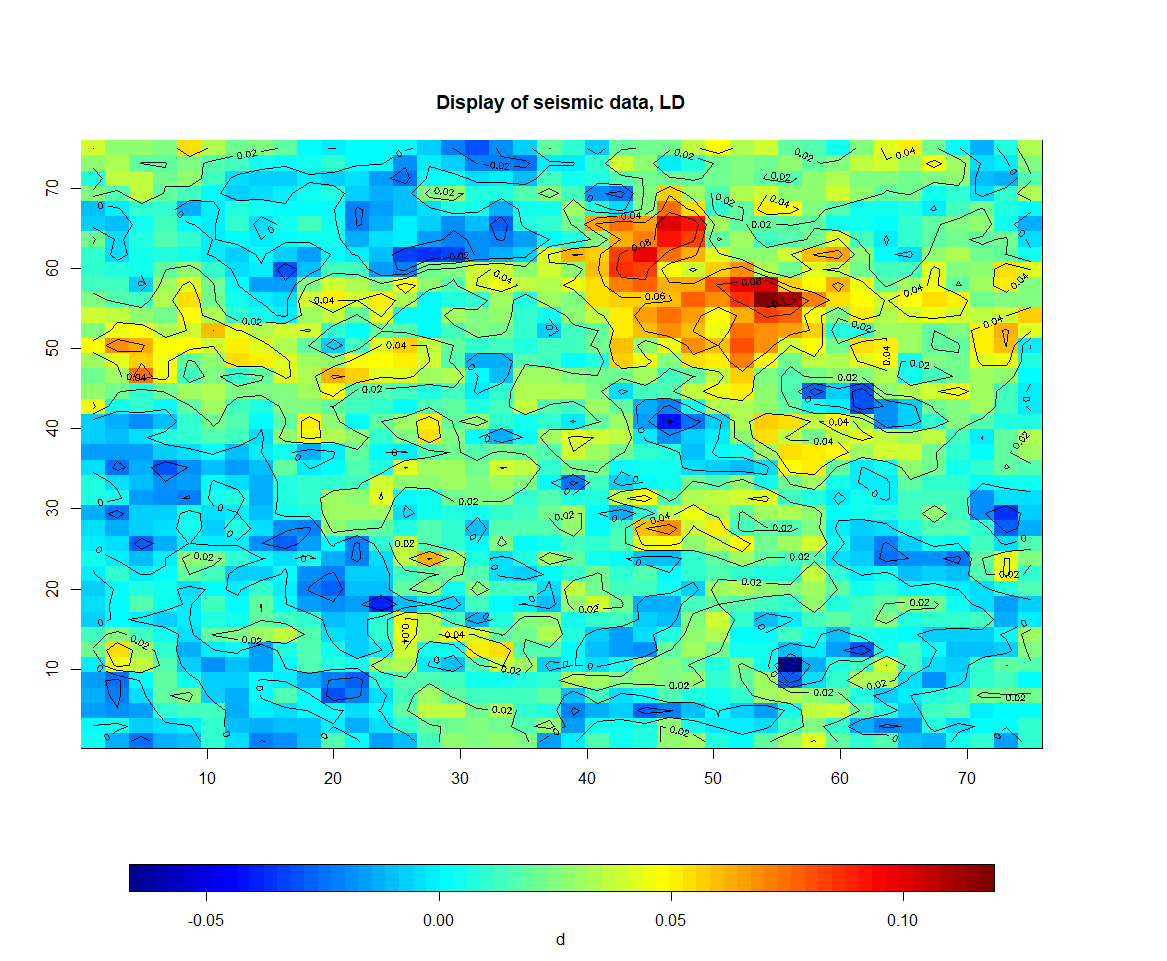
\includegraphics[scale=0.45]{figure1.png}
	 	\end{center}
	 	\caption{Display of seismic data $L_D$.}
	 	\label{fig:1a1} 
	\end{figure}
	 
	 
	 We display the observations from $L_D$ as a map in Figure \ref{fig:1a1}, there seems to be one large gathering where $d(\vect x)$ takes on relatively large values, there also seems to be some smaller gatherings of large $d(\vect x)$ in areas centered around the large one.  

	\newpage
	\subsection*{Problem 1b)}
	We now consider a uniform, independence prior model on $\vect l$. That will say: 
	\begin{equation}
		p(\vect l) = const
	\end{equation}
	We note that since the prior is constant we have:
	\begin{equation}
		p(\vect l | \vect d) \propto p(\vect d | \vect l)
	\end{equation}

	We get the following posterior model using bayes law and the law of total probability: 
	\begin{equation}
		p(\vect l | \vect d) = \dfrac{p(\vect d | \vect l)}{\sum_{\vect l \in \mathbb{L}^n}p(\vect d | \vect l)}
	\end{equation}
	Inserting from \eqref{eq:cond_prob} we get:
	\begin{equation}
		p(\vect l | \vect d) = \dfrac{ \prod_{i=1}^{n}  \phi(d_i |\mu = 0.02 + 0.06l_i, \sigma^2 = 0.06^2)}{\sum_{\vect l' \in \mathbb{L}^n} \prod_{i=1}^{n}  \phi(d_i |\mu = 0.02 + 0.06l_i', \sigma^2 = 0.06^2)}
	\end{equation}
	
	Where $\mathbb{L}^n$ is the n-dimensional space representing all possible values which $l$ can take. 

	As the prior is independent each point would also be conditional independent, for each point we thus get the following. Let: 
	\begin{equation}
		\begin{split}
		p_i &= p(l_i = 1 | d_i) 
		\\ &= \dfrac{p(d_i | l_i = 1)}{p(d_i | l_i = 0) + p(d_i | l_i = 1)}
		\\ &= \dfrac{\phi(d_i |\mu = 0.08, \sigma^2 = 0.06^2)}{\phi(d_i |\mu = 0.02, \sigma^2 = 0.06^2) + \phi(d_i |\mu = 0.08, \sigma^2 = 0.06^2)}
		\end{split}
	\end{equation}
	As each point either is sand or shale we get:
	\begin{equation}
		1 - p_i = p(l_i = 0 | d_i)
	\end{equation}
	We recognize this conditioned model as something Bernoulli-distributed with probability $p_i$. 
	
	We thus have: 
	\begin{equation}
		E(l_i | d_i) = p_i
	\end{equation}
	and 
	\begin{equation} \label{eq:var}
		Var(l_i | d_i) = p_i(1-p_i)
	\end{equation}
	
	\begin{figure}[h]	
		\begin{center} 
			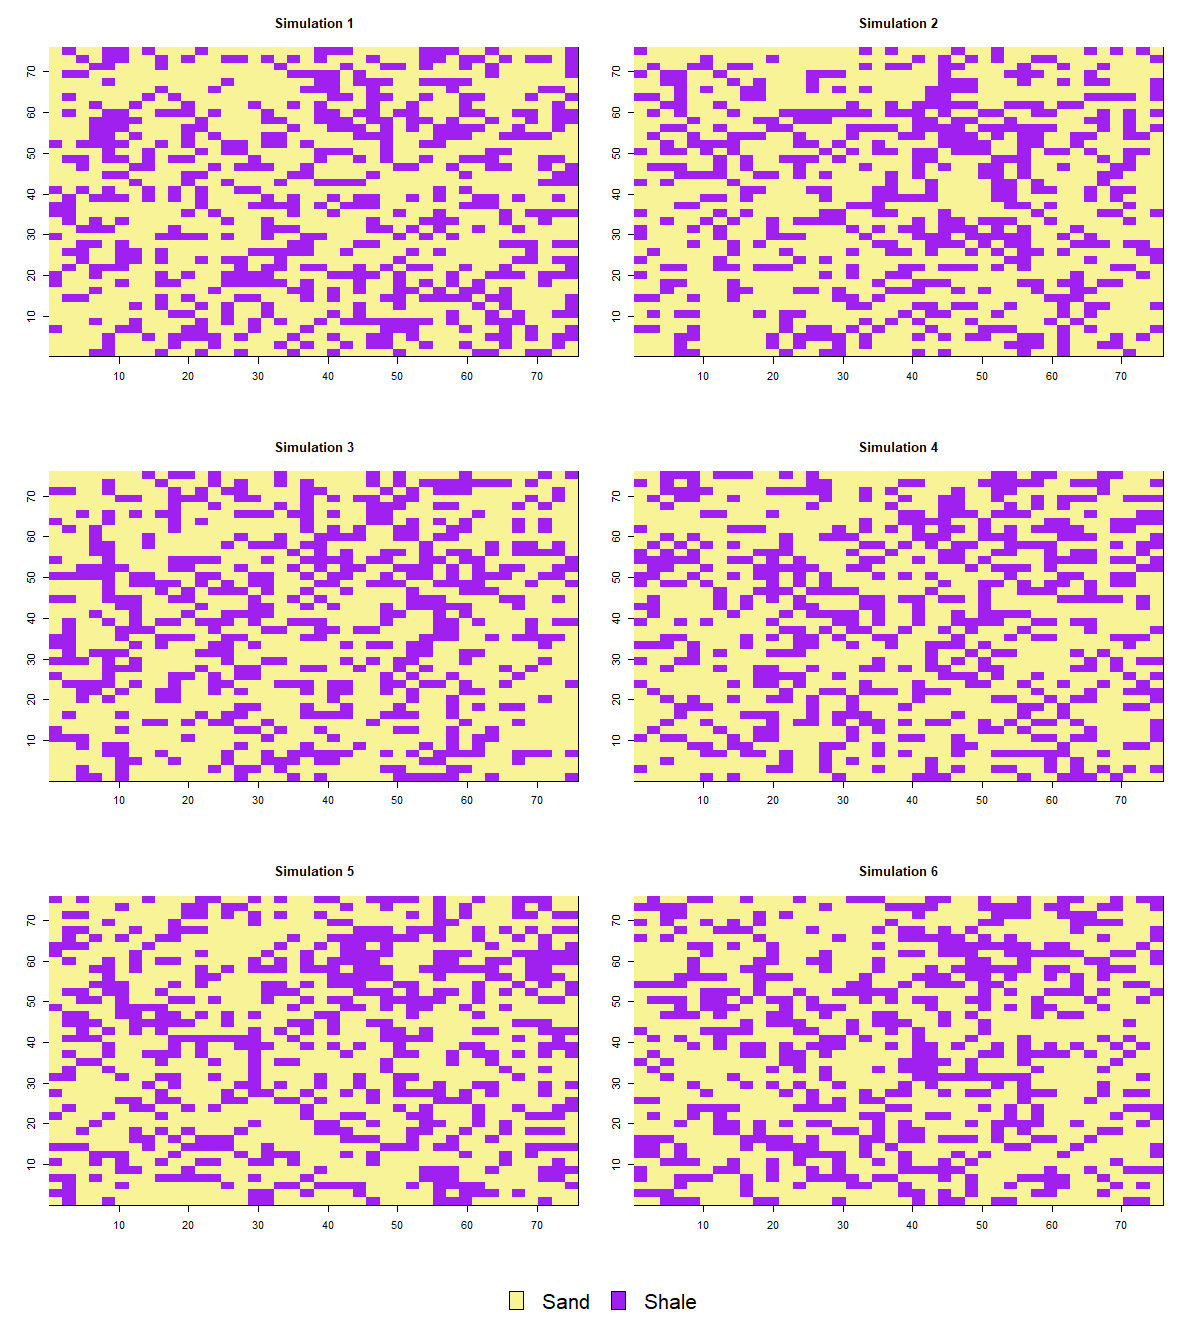
\includegraphics[scale=0.48]{figure2.png}
		\end{center}
		\caption{Display of six posterior realizations of $L_D$.}
		\label{fig:1b1} 
	\end{figure}
	
	
	We simulate 6 trials with the data and display the results in Figure \ref{fig:1b1}. 
	
	The maximum marginal posterior predictor ($MMAP\lbrace \vect l | \vect d \rbrace$) is defined as: 
	\begin{equation} \label{eq:mmap}
		MMAP\lbrace \vect l | \vect d \rbrace = \vect{\hat l} = argmax_{\vect l \in \mathbb{L}^n}\lbrace p(\vect l | \vect d)\rbrace
	\end{equation}
	
	Due to the conditional independence of the points we see: 
	\begin{equation}
		\hat l_i = \begin{cases}
		0, \text{ if } p_i < 0.5 \\
		1, \text{ if } p_i \geq 0.5
		\end{cases}
	\end{equation}
	Is a MMAP solution. 
		\begin{figure}[h]	
		\begin{center} 
			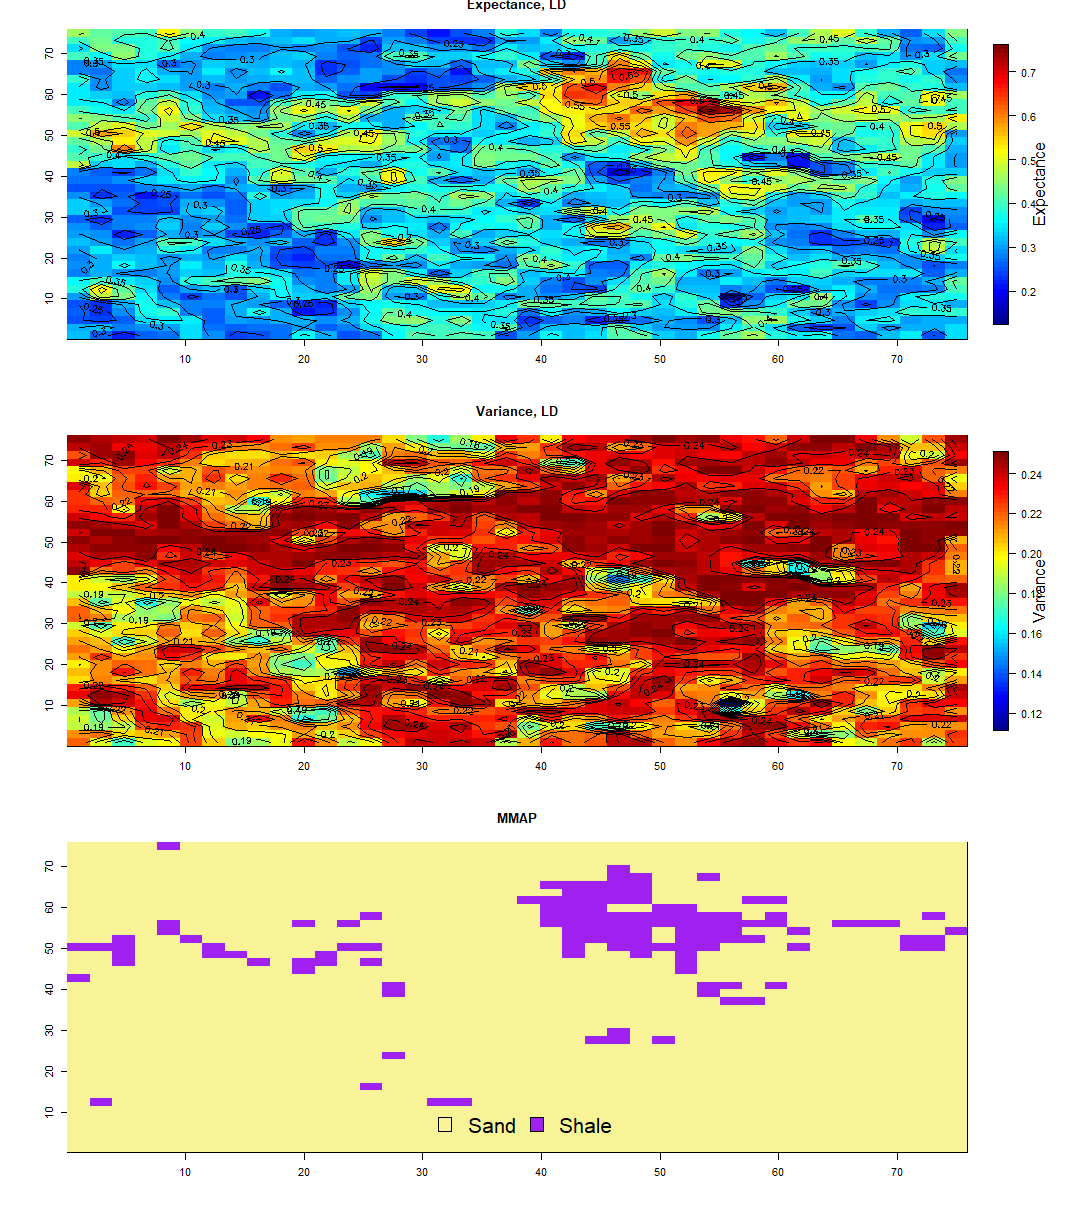
\includegraphics[scale=0.48]{figure4.png}
		\end{center}
		\caption{Display of six posterior realizations of $L_D$.}
		\label{fig:1b2} 
	\end{figure}
	
	We plot MMAP solution, expectance and variance in Figure \ref{fig:1b2}. We see that there is relatively high variance is most parts of the map, this is reflected in the large difference we see between the simulations. From both the expected value and the $MMAP$ we see that there is one large spot (top-right) where we expect a large cluster of shale as with some bands of shale on mid-left. This is somewhat reflected in the simulations. A difference betweeen MMAP and the simulations is that the simulations tend to expect more shale than the MMAP. The map of the expected values seems to be closer to the simulations than the MMAP. The MMAP result seems much less noisy. 
	
	\pagebreak
	\subsection*{Problem 1c)}
	Now consider a Markov RF prior model for $\lbrace l(\vect x); \vect x \in L_D \rbrace$. Represented by the n-vector $\vect l$ with the clique system $\vect c_L$ consisting of two closest neighbors on the grid $L_D$. 
	
	The corresponding Gibbs formulation is:
	\begin{equation}
		\begin{split}
		p(\vect l) = const \times \prod_{\vect c \in \vect c_L} v_{1l}(l_i, i \in \vect c) &= const \times \prod_{<i, j>\in L_D} \beta^{I(l_i = l_j)} \\
		&= const \times \beta^{\sum_{<i, j>\in L_D} I(l_i = l_j)}
		\end{split}
	\end{equation}
	With $<i, j> \in L_d$ defining the set of two closest neighbors on the grid $L_D$. 
	
	Want to find expressions for the posterior models and want to specify the Markov formulation for the Markov RF. 
	
	Want to find the Markov formulation for the Markov RF. First see:  
	\begin{equation}
		p(l_i | \vect l_{-i}) = \dfrac{p(\vect l)}{\sum_{l_i' \in \mathbb{L}} p(l_i', \vect l_{-i})} = \dfrac{p(\vect l)}{p(l_i = 1, \vect l_{-i}) +p(l_i = 0, \vect l_{-i})} 
 	\end{equation}
 	This reduces to: 
 	\begin{equation}
 		p(l_i | \vect l_{-i}) = p(l_i | l_j, j \in n_i)
 	\end{equation}
	
	We note that the joint distribution is given by:
	\begin{equation}
		\begin{split}
				p(\vect d, \vect l) &= p(\vect d | \vect l)p(\vect l) 
				\\ &= const \times \prod_{i=1}^{n}p(d_i | l_i) \prod_{\vect c \in \vect c_L} v_{1l}(l_i, i \in \vect c)
				\\ &= const \times \prod_{i=1}^{n}  \phi(d_i |\mu = 0.02 + 0.06l_i, \sigma^2 = 0.06^2) \prod_{<i, j>\in L_D} \beta^{I(l_i = l_j)}
		\end{split}
	\end{equation}
	
	We input the above into the following:
	\begin{equation}
		p(\vect l | \vect d) = \dfrac{p(\vect l, \vect d)}{p(\vect d)} = const  \times \prod_{i=1}^{n}  \phi(d_i |\mu = 0.02 + 0.06l_i, \sigma^2 = 0.06^2) \prod_{<i, j>\in L_D} \beta^{I(l_i = l_j)}
	\end{equation}
	Also: 
	\begin{equation}
	\begin{split}
		p(l_i, \vect d | \vect l_{-i}) &= p(\vect d | \vect l)p(l_i | \vect l_{-i}) \\ &= p(\vect d | \vect l)p(l_i | \vect l_{-i}) \\ 
		&= 	\dfrac{p(\vect l)}{p(l_i = 1, \vect l_{-i}) +p(l_i = 0, \vect l_{-i})} 	\prod_{i=1}^{n}  \phi(d_i |\mu = 0.02 + 0.06l_i, \sigma^2 = 0.06^2) 
	\end{split}
	\end{equation}
	Let $n_i$ be the neighborhood around the ith node. Then have:
	\begin{equation}
		p(l_i, \vect d | \vect l_{-i}) = \dfrac{\prod_{l_j \in n_i}\beta^{I(l_i = l_j)}}{\prod_{l_j \in n_i}\beta^{I(0 = l_j)} + \prod_{l_j \in n_i}\beta^{I(1 = l_j)}} 	\prod_{i=1}^{n}  \phi(d_i |\mu = 0.02 + 0.06l_i, \sigma^2 = 0.06^2) 
	\end{equation} 

	
	Now want to develop expressions for the posterior model  $p(l_i | \vect d, \vect l_{-i})$ have:
	\begin{equation}
		\begin{split}
		p(l_i | \vect d, \vect l_{-i}) &= p(l_i | d_i, l_{j} ; j \in n_i) 
		\\ &= \dfrac{p(l_i, d_i, l_j ; j \in n_i)}{p(d_i, l_j ; j \in n_i)}
		\\ &= \dfrac{p(d_i | l_i)\prod_{l_j \in n_i}\beta^{I(l_i = l_j)}}{\phi(d_i|\mu = 0.02, \sigma^2 = 0.06^2)\prod_{l_j \in n_i}\beta^{I(l_j = 0)} + \phi(d_i|\mu = 0.08, \sigma^2 = 0.06^2)\prod_{l_j \in n_i}\beta^{I(l_j = 1)}} 
		\end{split}		
	\end{equation} 
	
	as the Markov formulation. 
	
	\begin{figure}[h]	
		\begin{center} 
			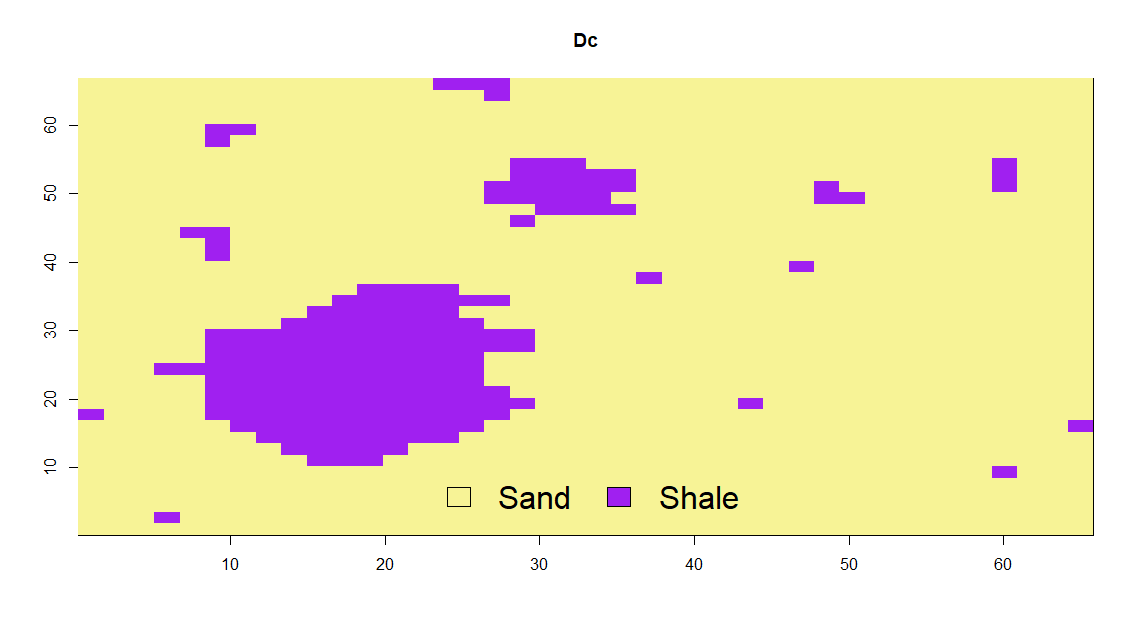
\includegraphics[scale=0.48]{figure5.png}
		\end{center}
		\caption{Display of observed data in $D_c$ }
		\label{fig:1c1} 
	\end{figure}

	We now display the observations in $D_c$ in Figure \ref{fig:1c1}.
	
	Now want to use these observations to estimate $\beta$ by a maximum pseudo-likelihood procedure. In a optimal solution we would use the assumed $p(\vect l)$ distribution to do this, however we would need $2^n$ calculations to evaluate the normalizing constant, which in our case is infeasible. We rather use the Markov formulation to create an approximation.  (here $\vect d \in \mathbb{L}^n$)
	
	\begin{equation} \label{eq:ising}
		p(\vect d | \beta ) \approx \hat p(\vect d | \beta) = const \times \prod_{i = 1}^{n}\sum_{\lbrace l_i', l_j' | l_j' \in n_i \rbrace \in L }  \prod_{j = i, j \in n_i}p(d_j | l_j')p(l_i'|l_j')
	\end{equation}
	

	
	As we assume the observations to $\vect l$ from $D_c$ be exact the model reduces as:
	\begin{equation}
	p(d_i | l_i') \rightarrow \delta_{d_i}(l_i') = \begin{cases}
		1, l_i' = l_i \\ 
		0, \text{ else}
		\end{cases}
	\end{equation} 
	
	This reduces \eqref{eq:ising} to: 
	\begin{equation}
		\hat p(\vect d | \beta) \propto \prod_{i = 1}^n p(d_i|l_j; j \in n_i; \beta) = \prod_{i=1}^{n}\dfrac{\beta^{\sum_{j \in n_i}I(l_i = l_j)}}{\beta^{\sum_{j \in n_i}I(0 = l_j)} + \beta^{\sum_{j \in n_i}I(1 = l_j)}}
	\end{equation}
	
	A good estimation of $\beta$ would be to maximize the above giving:
	\begin{equation}
		\hat \beta = \text{argmax}_\beta \sum_{i=1}^{n} \left\{ \left( \sum_{j \in n_i}I(l_i = l_j)\right)\log\beta - \log\left(\beta^{\sum_{j \in n_i}I(0 = l_j)} + \beta^{\sum_{j \in n_i}I(1 = l_j)}\right) \right\}
	\end{equation}
	
	Using the Optim function in R this value can be "easily" found.  Implementing the function and running we get that $\hat \beta \approx 3.46$.
	
	We can use the information we learned from $D_c$ and apply it to out model on $L_d$ as their lithology is comparable. 
	
	Focus is on realizations from $p(\vect l|\vect d)$, with related predictions $E(\vect l|\vect d)$, variances
	in the diagonal terms of $Var(\vect l|\vect d)$, and alternative predictions $MMAP(\vect l|\vect d)$.
	
	To estimate these, we use a MCMC/Gibbs algorithm with a single-site proposal based on the Markov formulation for the Markov RF. The pseudocode for the algorithm is given below. 
	\begin{algorithm}[H]
	\caption{MCMC/Gibbs algorithm for $p(\vect l| \vect d)$ realizations }
	\begin{algorithmic}
		\STATE{$\beta = \hat \beta$}
		\STATE{$\vect l^0 = p(\vect  l^0 | \vect d) > 0$}
		\FORALL{$j = 1,  2, ...$}
			\STATE{$\vect l^j \sim g(\vect l | \vect l^{j-1})$}
		\ENDFOR	
\end{algorithmic}
\end{algorithm}

	
	\begin{algorithm}[H]
		\caption{Function $g(\vect l' | \vect l)$ }
		\begin{algorithmic}
			\STATE{$i \sim Uniform(1, ..., n)$}
			\STATE{$l_i' \sim p(l_i | d_i, l_j, j \in n_i)$} 
			\STATE{$\vect l' = (l_1, ..., l_{i-1}, l_i', l_{i+1}, ..., l_n)$}
			\STATE{return $\vect l'$}
		\end{algorithmic}
	\end{algorithm}

\begin{figure}[h]	
	\begin{center} 
		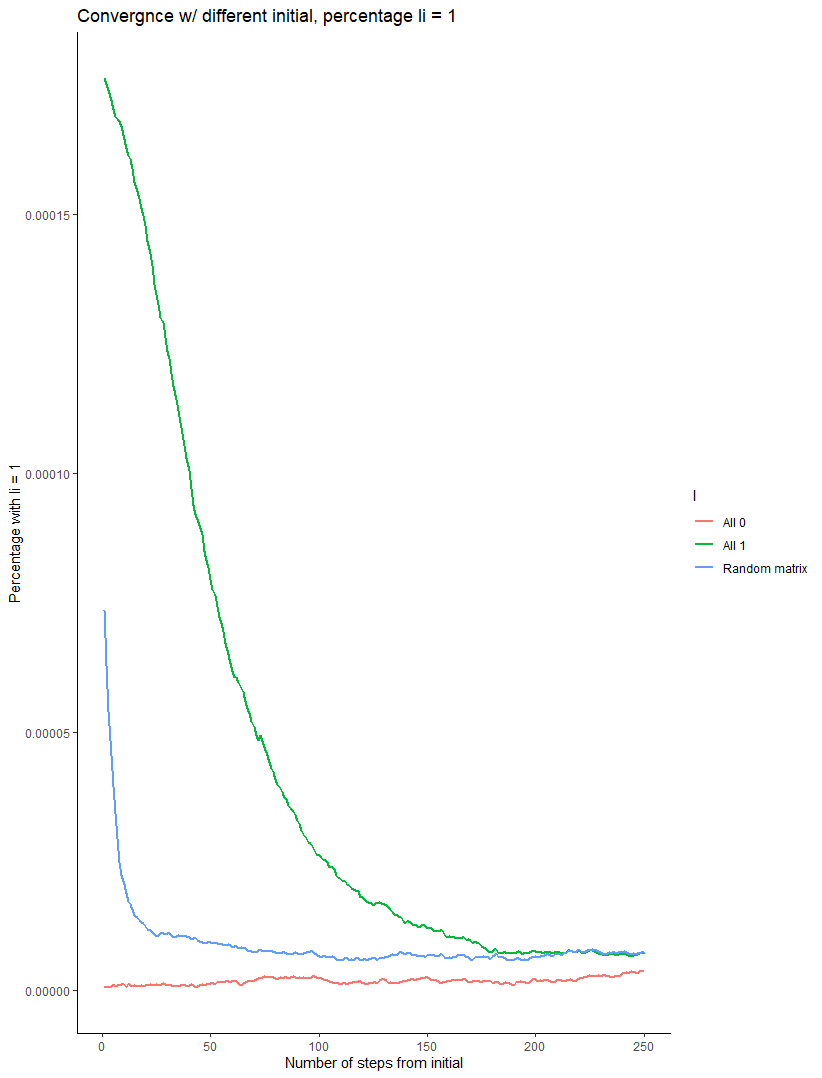
\includegraphics[scale=0.48]{plotc1.png}
	\end{center}
	\caption{Gibbssampler convergence, percentage of $l_i$-s that are zero. With $\hat \beta = 3.46$. }
	\label{fig:c1} 
\end{figure}

\begin{figure}[h]	
	\begin{center} 
		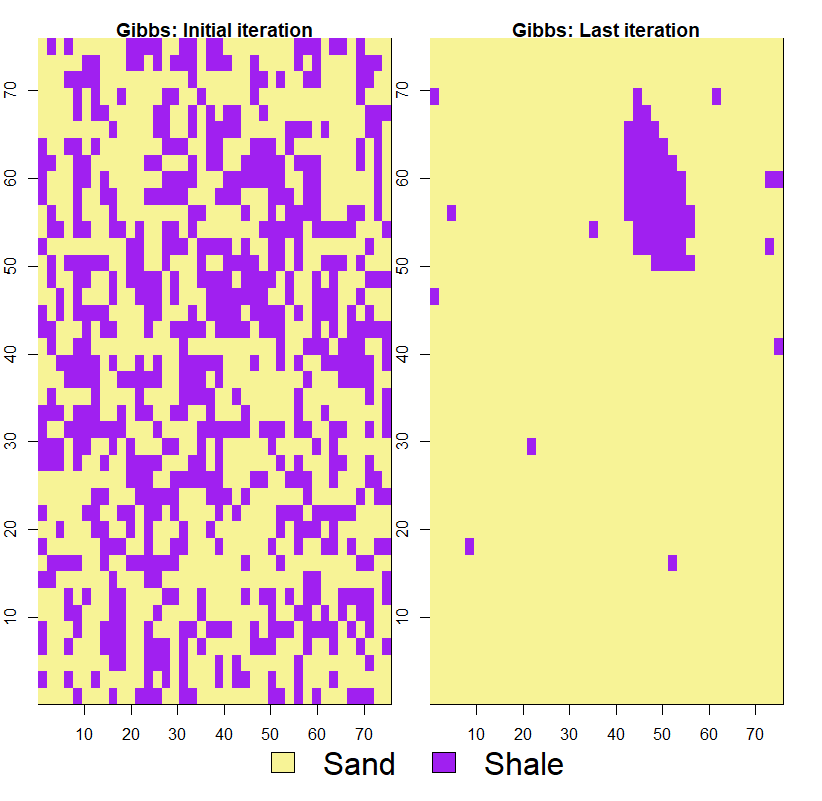
\includegraphics[scale=0.48]{c2.png}
	\end{center}
	\caption{Gibbssampler first at last iteration, 2500 steps.}
	\label{fig:c2} 
\end{figure}




We implement and run the algorithm for three different initial values. One where we start with $\vect l$ as all zeroes. One where we start with $\vect l$ as all ones. And one where $\vect l$ elements are randomly 1 or 0 with equal chance for each. To check convergence we plot percentage of $l_i$-s that are 1 compared to iteration numbers. The results are displayed in figure \ref{fig:c1}. We run the sampler for 250 iterations in each case. We see that the sampler starting at all 0 and all 1 meet after about 200 iterations we thus assume that they have converged. The random start reach this point the fastest, and seems to keep stationary after about 50 iterations. The one with all ones take 4 times as many iterations to reach the same point. The sampler starting at all 0 seems to slowly move towards the two others, but have not managed to do so after 250 iterations. We conclude that it is best to start with the random matrix. 

To simulate realizations we run 2500 iterations with the sampler starting with the random matrix. We assume burnin after 50 iterations. After that we take each sweep as a sample (we disregard correlation between close samples to keep our method simple). First and last iteration is displayed in Figure \ref{fig:c2}. 

\begin{figure}[h]	
	\begin{center} 
		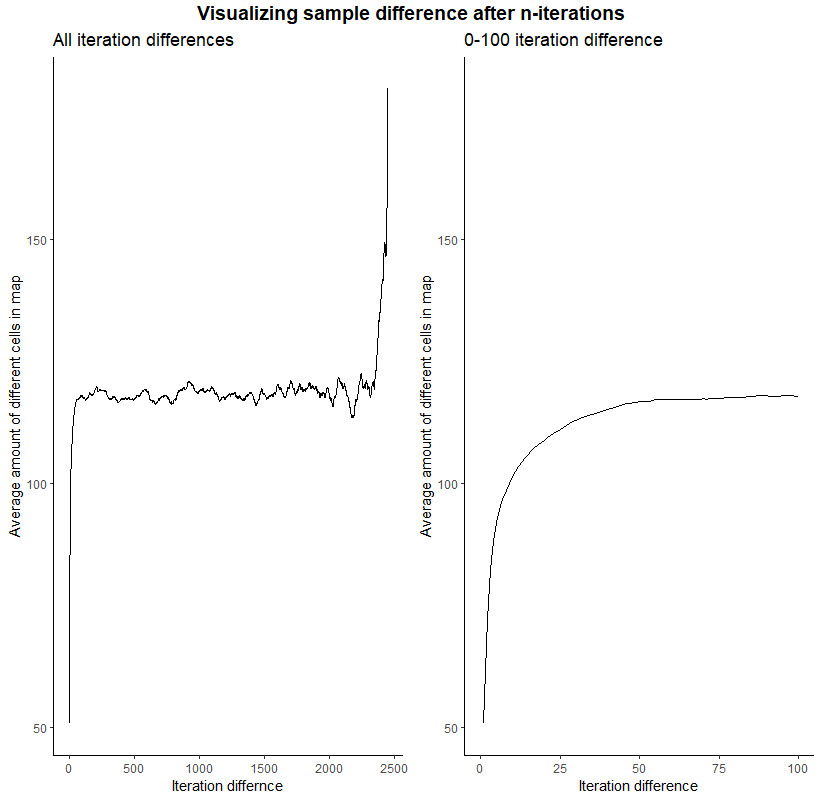
\includegraphics[scale=0.48]{c3.png}
	\end{center}
	\caption{Average sample difference, 2450 samples, to check independence}
	\label{fig:c3} 
\end{figure}

To control for sample independence, we calculate how many different cells we have between each cell in the sample after removing burnin. We then plot the average iteration difference. This is displayed in Figure \ref{fig:c3}. After about 50 iterations the difference seems to be stablizing at approximately 110 different cells in each map. So we thus take every 50-th step as a independent sample.  

Using our independent samples we have following estimator:
\begin{equation}
	E(l_i|d_i) = p_i = \dfrac{1}{m}\sum_{j=1}^ml_i^j
\end{equation}


\begin{figure}[h]	
	\begin{center} 
		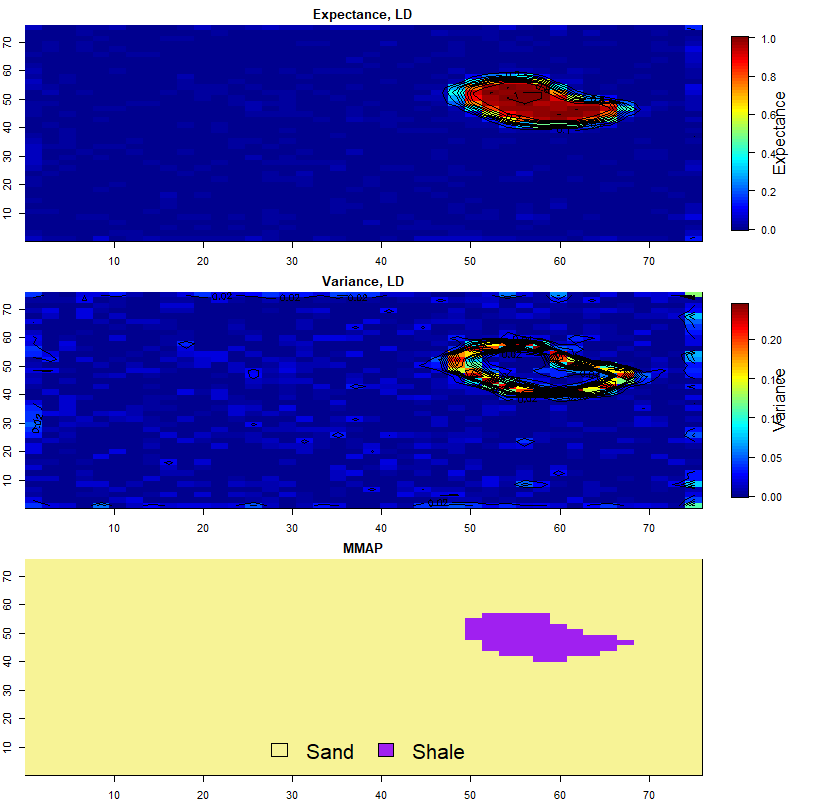
\includegraphics[scale=0.75]{c4.png}
	\end{center}
	\caption{Estimators from independent gibbs samples}
	\label{fig:c4} 
\end{figure}


Where $m$ is the number of independent samples, and $l_i^j$ is the $i$-th cell in the $j$-th sample.
Estimators for variancce and MMAP are \eqref{eq:var} and \eqref{eq:mmap} respectively.  The results hare shown in Figure \ref{fig:c4}. 
Compared with the model with the constant prior this model gives a result with a solid body, in the top-right part of the plot. Variance is close to zero, expect at the edges of the solid shale area. The MMAP reflects the expected value, and only shows one connected area where one expect shale. 


\end{document}